\documentclass{article}
\usepackage{graphicx} % Required for inserting images
\usepackage{lmodern}        % Latin Modern family of fonts
\usepackage[T1]{fontenc}
\usepackage[utf8]{inputenc}
\usepackage{listings}
\usepackage{color}

\title{Deep Learning Task1 Report}
\author{DHYEY ITALIYA\\ABIR ABHYANKAR}
\date{March 2024}

\begin{document}

\maketitle

\section{Data Preparation}
We were initially given an audio dataset, with varied audio lengths. Some of the files were not formatted correctly, while some were with the wrong extension.\\

The dataset had audio clips which were of a maximum length of 4 seconds. To handle the problem of varying audio lengths, we resized all the audio files to 4 seconds, by padding the audio files with silence.\\

For files which were not formatted properly, we converted them into \textbf{.wav} files, which we then used further. Files with the wrong extension were individually identified and corrected.\\

With these standardised audio files, we generated their Mel-Spectrograms using the \textbf{librosa} library in python. Mel-Spectrograms capture the most essential features of the audio files are often the most suitable way to input audio data into deep learning models. \\

Our CNN models have been trained on the Mel-Spectrograms.
%---------------------------------------- ---------------------------------
\section{Choice of Models}
The two models chosen by our team is Inception v-1 Network (GoogleNet) and Residual Networks.
%--------
\subsection{Inception v-1 (GoogleNet)}
GoogleNet introduced the concept of "Inception modules," which are essentially multiple parallel convolutional layers of different filter sizes followed by pooling operations. These modules allow the network to capture features at multiple scales efficiently, enabling better representation learning. This allows teh model to have comparable performance with other CNN architectures with considerably less parameters, thus leading to faster training time\\

Despite its depth, GoogleNet is computationally efficient compared to other deep neural networks like VGGNet or AlexNet. This efficiency is achieved through the use of 1x1 convolutions, which reduce the number of computations required while maintaining model performance.\\

Instead of fully connected layers at the end of the network, GoogleNet utilizes global average pooling (GAP) to reduce overfitting and the number of parameters. GAP computes the average of each feature map and directly connects it to the output layer.This approach reduces the number of parameters and makes the network more robust to spatial translations of the input.\\


GoogleNet's design principles focus on achieving a good balance between model complexity, computational efficiency, and performance, making it a popular choice for image tasks, especially when computational resources are limited.\\
%-----------
\subsection{Residual Networks}

The fundamental building blocks of ResNet are residual blocks, which consist of shortcut connections (also known as skip connections) that bypass one or more convolutional layers. These connections allow the network to learn residual mappings instead of directly learning the desired underlying mapping. By learning residuals, the network can be trained more effectively, especially for very deep architectures. This alleviates the vanishing gradient problem and facilitates the training of extremely deep networks.\\

The skip connections in ResNet provide an alternate path for gradients during back-propagation, mitigating the vanishing gradient problem. This enables more efficient training by ensuring that gradients can flow through the network without significant attenuation, even in very deep architectures.\\

Pre-trained ResNet models, trained on large datasets like ImageNet, are readily available and can be fine-tuned or used as feature extractors for various image-related tasks. This facilitates transfer learning, where knowledge learned from one task (e.g., image classification) can be transferred to another related task (e.g., object detection, segmentation) with relatively little additional training data.\\

Overall, ResNet's innovative use of residual connections and its ability to train very deep networks effectively have made it a popular choice for image tasks, achieving state-of-the-art performance in various benchmarks and competitions.
%-----------------------------------------------------------------------------
\section{Training}
Firstly the generated spectrograms are transformed using \texttt{torchvision.transforms} where the image is resized to 224*224 and converted to tensor.\\
\begin{lstlisting}
transform = transforms.Compose([
    transforms.Resize((224, 224)),
    transforms.ToTensor()
])
\end{lstlisting}

The batch size used for the train and test dataloader is 64. Experiments we performed with batch size of 32, 64 and 128. Best performance was observed in case of \texttt{batch\_size = 64}.\\

The loss function used is cross-entropy loss. The optimizer used is Adam for both models. However, the learning rate is different between the two models. For Resnet training, the initial learning rate is 0.001; for GoogleNet, the initial learning rate is 0.0001. This difference is because Resnet has more parameters and can easily leverage the higher learning rate. The weight decay for both the parameters is 0.0001.\\

By experimentation, we found that using a learning rate scheduler helped achieve faster and better convergence; however, this is optional in the case of Adam Optimiser.\\

While training both the models were trained for 45 epochs and then after that the the learning rate is reduced by factor of 10 and trained for 20 epochs. This is done in order to converge the model to lowest loss.\\

On Validation dataset, following are the performance metrics:
\begin{enumerate}
\item GoogleNet Based Model

\begin{itemize}

\item
Training Time - \textbf{40 - 45 Minutes}
\item 
Number of Parameters - $10339607$

\end{itemize}
\begin{lstlisting}
Accuracy: 0.9122
Precision: 0.9146
Recall: 0.9122
F1 Score: 0.9101
\end{lstlisting}

\item ResNet Based Model

\begin{itemize}
\item
Training Time - \textbf{90 - 100 Minutes}
\item
Number of Parameters - $22676109$
\end{itemize}
\begin{lstlisting}
Accuracy = 0.9401
Precision = 0.9400
Recall = 0.9401
F-1 Score = 0.9398
\end{lstlisting}
\end{enumerate}
\\
You can find the validation accuracy and loss curves along with the confusion matrices for both models after the \textbf{Trials} section.

\section{Trials}

We mainly tried 2 data augmentation and pre-processing techniques.\\

\textbf{Technique 1} - Given the nature of the dataset, we reasoned that instead of simply padding the audio file with silence, we could loop the audio file, so the model could better grasp the features of the audio, but this method had a lower accuracy than just padding with silence.\\

\textbf{Technique 2} - The method we used in the final model is simple, and just resizes the audio file by padding with silence, without any looping.\\

Provided below is a performance metrics comparison between the 2 techniques, when they were applied on the GoogleNet Architecture.

\begin{lstlisting}
    Technique 1                     Technique 2
    Accuracy: 0.8267                Accuracy: 0.9122
    Precision: 0.8458               Precision: 0.9146
    Recall: 0.8267                  Recall: 0.9122
    F1 Score: 0.8288                F1 Score: 0.9101
\end{lstlisting}\\

We also tried training with multiple batch-sizes as mentioned in the \textbf{Training} Section, where we found that the batch-size of 64 worked best for the models.

\section{Curves and Plots}
% Paste the val_acc_history and loss_history plots
\begin{figure}[!hp]
  \centering
  \begin{minipage}[b]{\textwidth}
    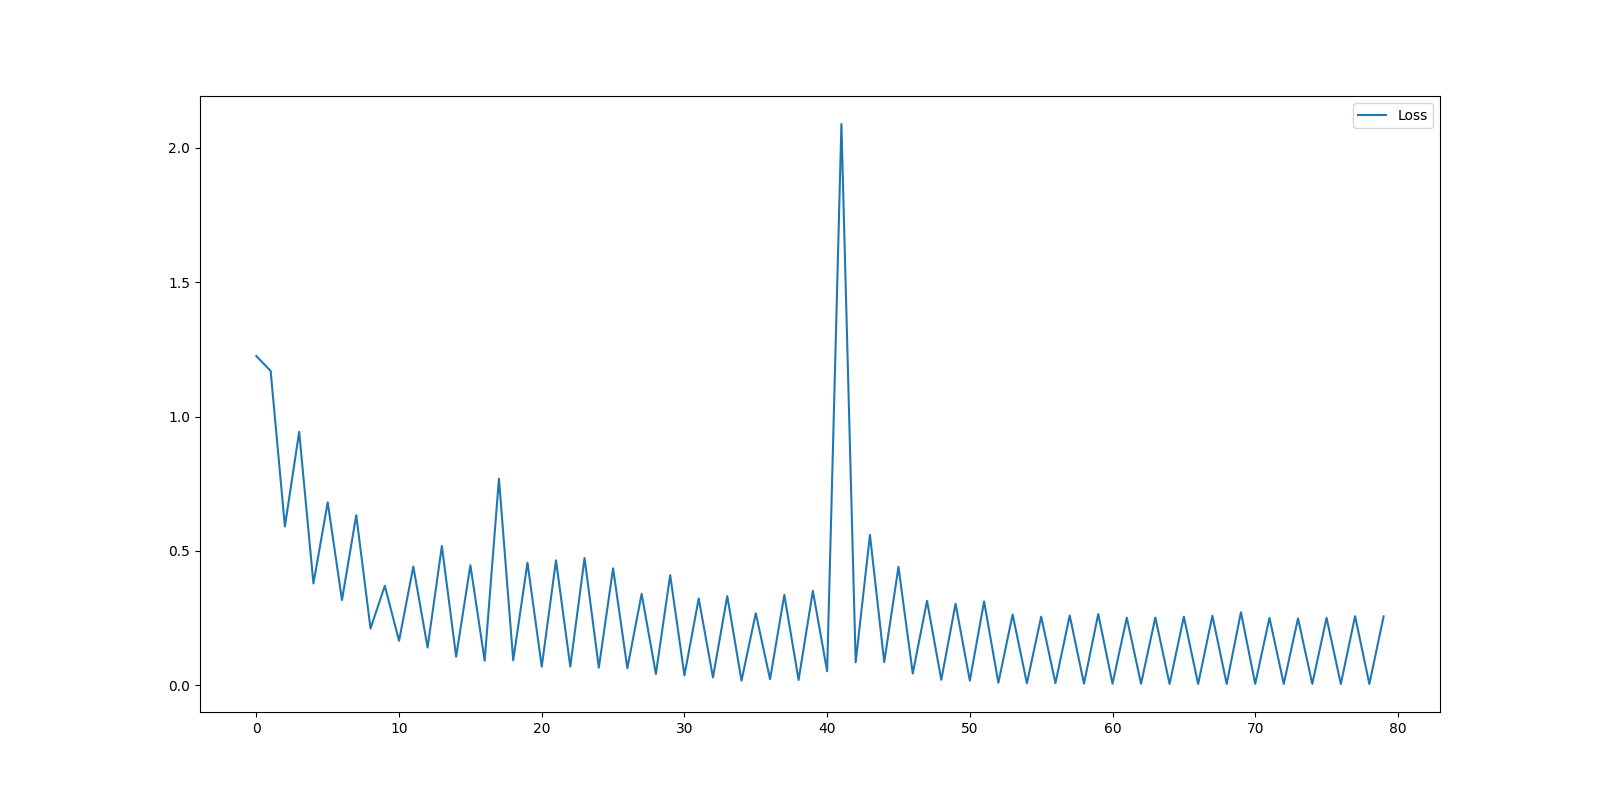
\includegraphics[width=\textwidth]{loss_history_RN.png}
    \caption{Training Loss for ResNet}
  \end{minipage}
  \hfill
  \begin{minipage}[b]{\textwidth}
    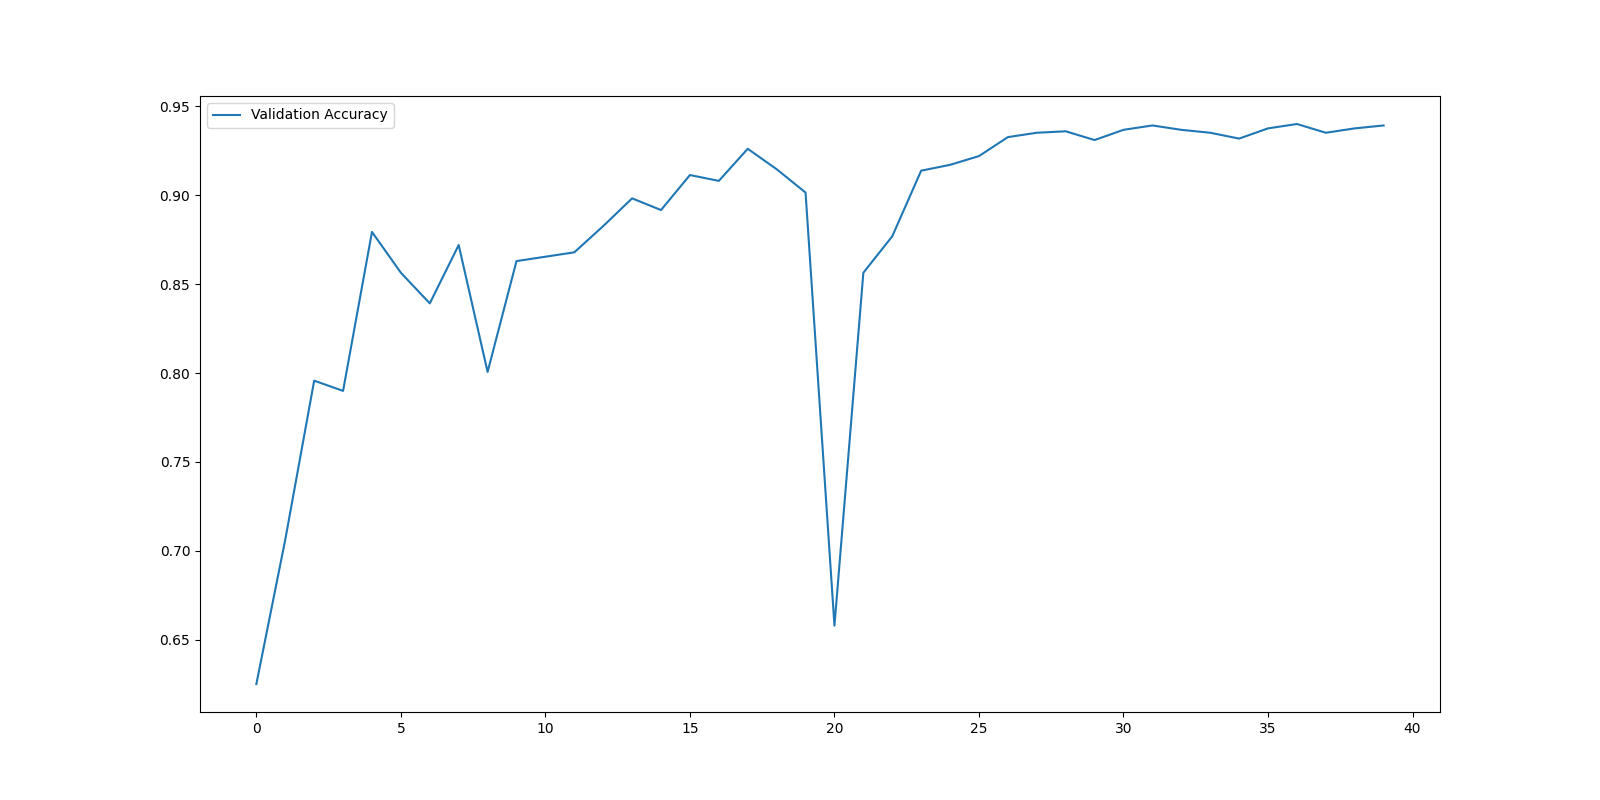
\includegraphics[width=\textwidth]{val_acc_history_RN.png}
    \caption{Validation Accuracy for ResNet}
  \end{minipage}
\end{figure}

% Paste the val_acc_history and loss_history plots
\begin{figure}[!hp]
  \centering
  \begin{minipage}[b]{\textwidth}
    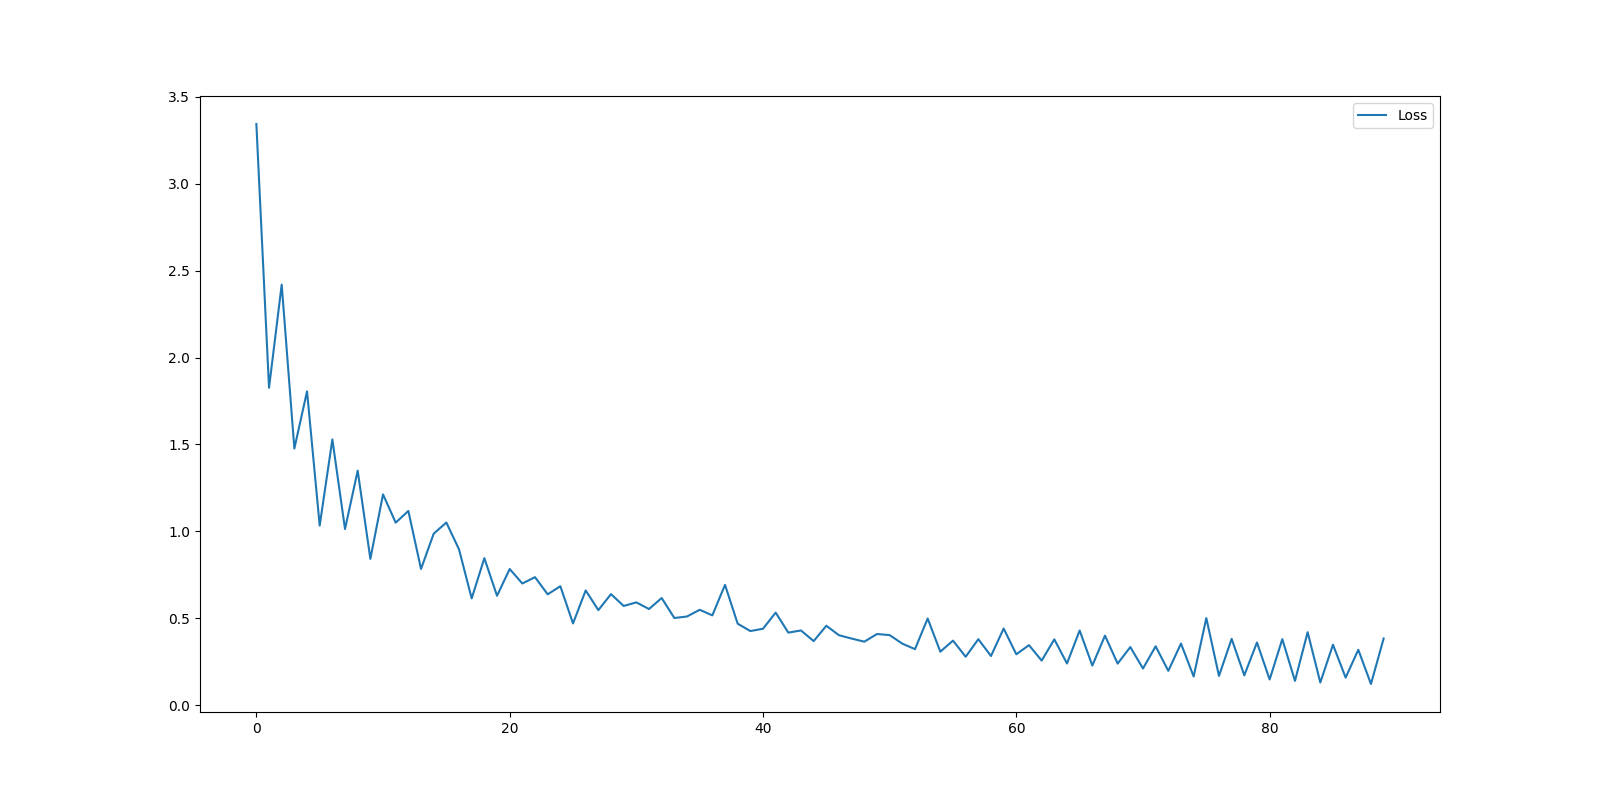
\includegraphics[width=\textwidth]{loss_history_GN.png}
    \caption{Training Loss for GoogleNet}
  \end{minipage}
  \hfill
  \begin{minipage}[b]{\textwidth}
    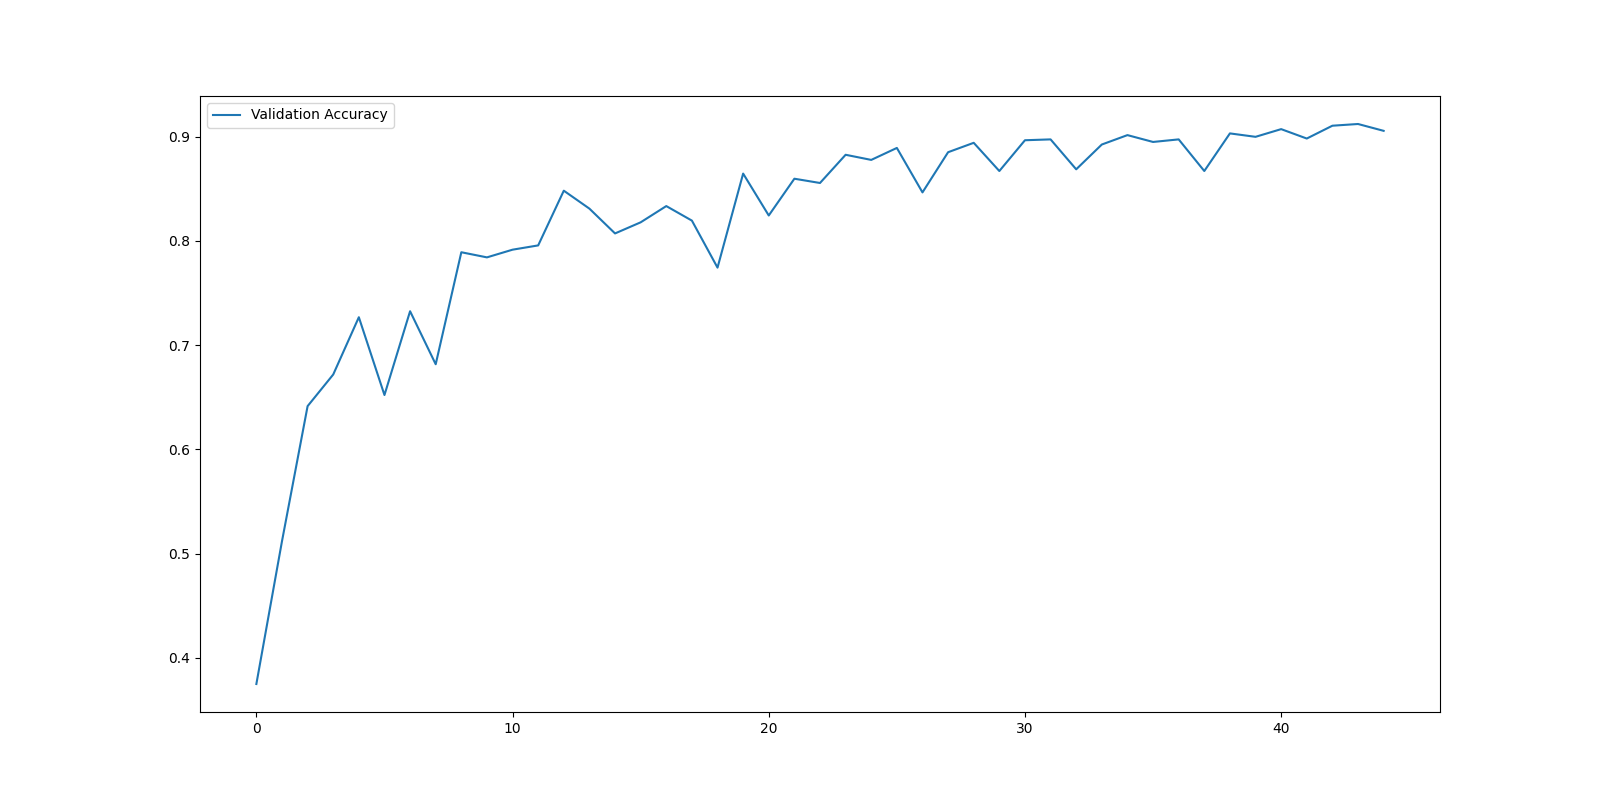
\includegraphics[width=\textwidth]{val_acc_history_GN.png}
    \caption{Validation Accuracy for GoogleNet}
  \end{minipage}
\end{figure}

%paste the confusion matrix images

\begin{figure}[!hp]
  \centering
  \begin{minipage}[b]{\textwidth}
    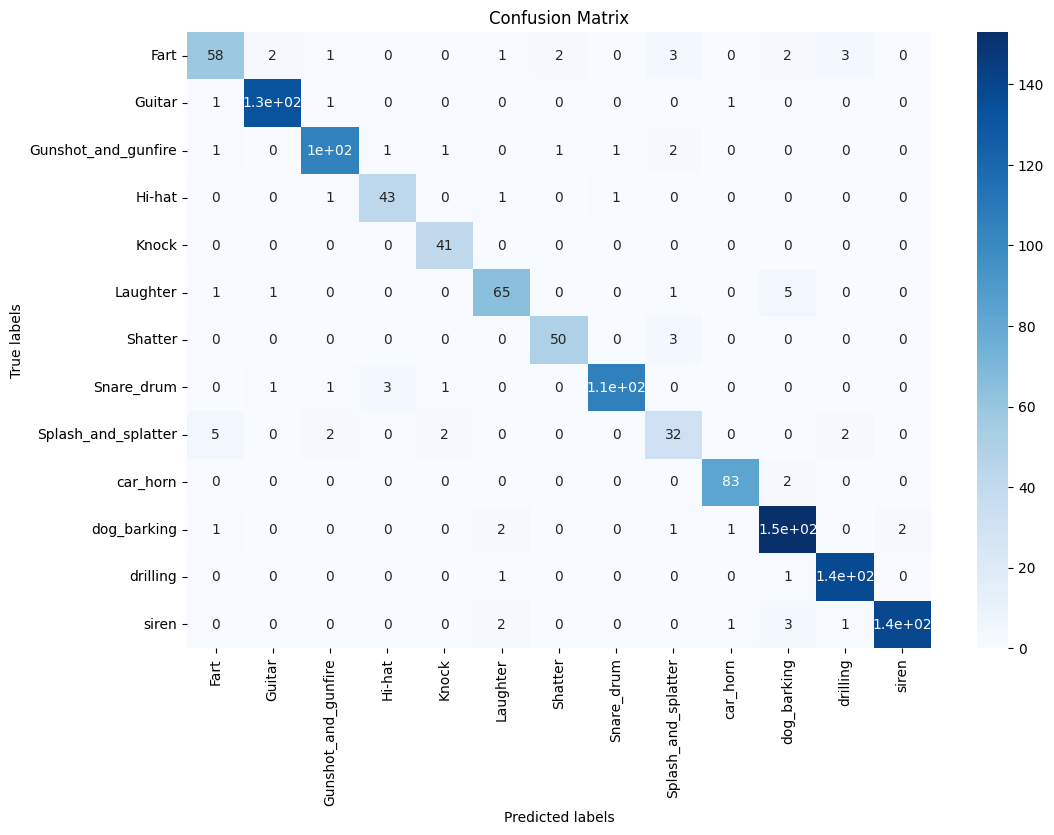
\includegraphics[width=\textwidth]{conf_RN.png}
    \caption{Confusion Matrix ResNet}
  \end{minipage}
  \hfill
\end{figure}

\begin{figure}[!hp]
  \centering
  \begin{minipage}[b]{\textwidth}
    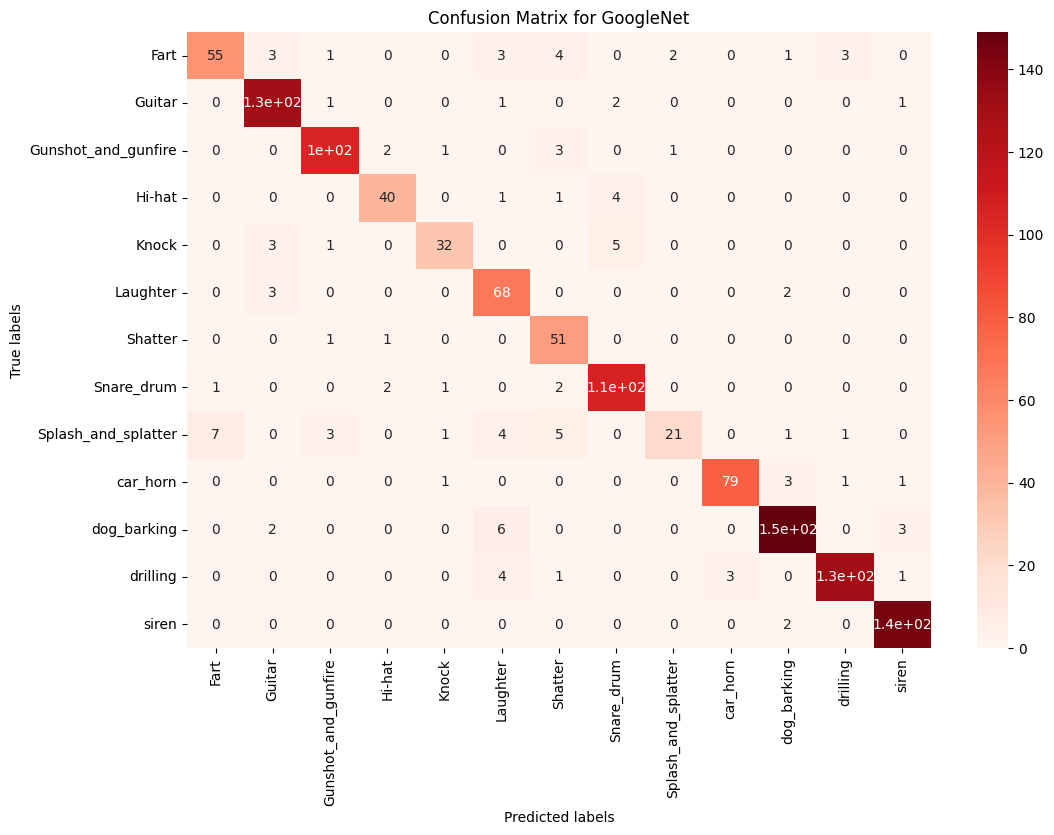
\includegraphics[width=\textwidth]{conf_GN.png}
    \caption{Confusion Matrix GoogleNet}
  \end{minipage}
  \hfill
\end{figure}

%---------------------------------------------------------------------------

\end{document}


